% Options for packages loaded elsewhere
% Options for packages loaded elsewhere
\PassOptionsToPackage{unicode}{hyperref}
\PassOptionsToPackage{hyphens}{url}
\PassOptionsToPackage{dvipsnames,svgnames,x11names}{xcolor}
%
\documentclass[
  10pt,
  letterpaper,
  oneside,
  open=any]{scrbook}
\usepackage{xcolor}
\usepackage[bindingoffset=0.0in,left=24mm,top=24mm,bottom=24mm,right=24mm]{geometry}
\usepackage{amsmath,amssymb}
\setcounter{secnumdepth}{-\maxdimen} % remove section numbering
\usepackage{iftex}
\ifPDFTeX
  \usepackage[T1]{fontenc}
  \usepackage[utf8]{inputenc}
  \usepackage{textcomp} % provide euro and other symbols
\else % if luatex or xetex
  \usepackage{unicode-math} % this also loads fontspec
  \defaultfontfeatures{Scale=MatchLowercase}
  \defaultfontfeatures[\rmfamily]{Ligatures=TeX,Scale=1}
\fi
\usepackage{lmodern}
\ifPDFTeX\else
  % xetex/luatex font selection
\fi
% Use upquote if available, for straight quotes in verbatim environments
\IfFileExists{upquote.sty}{\usepackage{upquote}}{}
\IfFileExists{microtype.sty}{% use microtype if available
  \usepackage[final]{microtype}
  \UseMicrotypeSet[protrusion]{basicmath} % disable protrusion for tt fonts
}{}
\makeatletter
\@ifundefined{KOMAClassName}{% if non-KOMA class
  \IfFileExists{parskip.sty}{%
    \usepackage{parskip}
  }{% else
    \setlength{\parindent}{0pt}
    \setlength{\parskip}{6pt plus 2pt minus 1pt}}
}{% if KOMA class
  \KOMAoptions{parskip=half}}
\makeatother
% Make \paragraph and \subparagraph free-standing
\makeatletter
\ifx\paragraph\undefined\else
  \let\oldparagraph\paragraph
  \renewcommand{\paragraph}{
    \@ifstar
      \xxxParagraphStar
      \xxxParagraphNoStar
  }
  \newcommand{\xxxParagraphStar}[1]{\oldparagraph*{#1}\mbox{}}
  \newcommand{\xxxParagraphNoStar}[1]{\oldparagraph{#1}\mbox{}}
\fi
\ifx\subparagraph\undefined\else
  \let\oldsubparagraph\subparagraph
  \renewcommand{\subparagraph}{
    \@ifstar
      \xxxSubParagraphStar
      \xxxSubParagraphNoStar
  }
  \newcommand{\xxxSubParagraphStar}[1]{\oldsubparagraph*{#1}\mbox{}}
  \newcommand{\xxxSubParagraphNoStar}[1]{\oldsubparagraph{#1}\mbox{}}
\fi
\makeatother


\usepackage{longtable,booktabs,array}
\usepackage{calc} % for calculating minipage widths
% Correct order of tables after \paragraph or \subparagraph
\usepackage{etoolbox}
\makeatletter
\patchcmd\longtable{\par}{\if@noskipsec\mbox{}\fi\par}{}{}
\makeatother
% Allow footnotes in longtable head/foot
\IfFileExists{footnotehyper.sty}{\usepackage{footnotehyper}}{\usepackage{footnote}}
\makesavenoteenv{longtable}
\usepackage{graphicx}
\makeatletter
\newsavebox\pandoc@box
\newcommand*\pandocbounded[1]{% scales image to fit in text height/width
  \sbox\pandoc@box{#1}%
  \Gscale@div\@tempa{\textheight}{\dimexpr\ht\pandoc@box+\dp\pandoc@box\relax}%
  \Gscale@div\@tempb{\linewidth}{\wd\pandoc@box}%
  \ifdim\@tempb\p@<\@tempa\p@\let\@tempa\@tempb\fi% select the smaller of both
  \ifdim\@tempa\p@<\p@\scalebox{\@tempa}{\usebox\pandoc@box}%
  \else\usebox{\pandoc@box}%
  \fi%
}
% Set default figure placement to htbp
\def\fps@figure{htbp}
\makeatother





\setlength{\emergencystretch}{3em} % prevent overfull lines

\providecommand{\tightlist}{%
  \setlength{\itemsep}{0pt}\setlength{\parskip}{0pt}}



 


\usepackage{xcolor}
\usepackage{sectsty}
\usepackage{titlesec}
\definecolor{customnavy}{RGB}{0, 0, 128}
\sectionfont{\color{customnavy}}
\subsectionfont{\color{customnavy}}   
\subsubsectionfont{\color{customnavy}}   
\usepackage{amssymb}
\usepackage{pifont}
\usepackage{wasysym}
\usepackage{fontawesome5}
\usepackage{etoolbox}
\makeatletter
\patchcmd{\scr@startchapter}{\if@openright\cleardoublepage\else\clearpage\fi}{}{}{}
% Adjust spacing before and after headings
\usepackage{titlesec}
\titleformat{\section}
  {\normalfont\Large\bfseries\color{customnavy}\centering} % Format
  {} % Label (empty = no number)
  {0pt} % Separation between label and title
  {} % Before-code

\titlespacing*{\section}{0pt}{0pt}{0pt}      % {left}{before}{after}
\titlespacing*{\subsection}{0pt}{2pt}{2pt}   % {left}{before}{after}
\titlespacing*{\subsubsection}{0pt}{2pt}{2pt}   % {left}{before}{after}
\makeatletter
\@ifpackageloaded{tcolorbox}{}{\usepackage[skins,breakable]{tcolorbox}}
\@ifpackageloaded{fontawesome5}{}{\usepackage{fontawesome5}}
\definecolor{quarto-callout-color}{HTML}{909090}
\definecolor{quarto-callout-note-color}{HTML}{0758E5}
\definecolor{quarto-callout-important-color}{HTML}{CC1914}
\definecolor{quarto-callout-warning-color}{HTML}{EB9113}
\definecolor{quarto-callout-tip-color}{HTML}{00A047}
\definecolor{quarto-callout-caution-color}{HTML}{FC5300}
\definecolor{quarto-callout-color-frame}{HTML}{acacac}
\definecolor{quarto-callout-note-color-frame}{HTML}{4582ec}
\definecolor{quarto-callout-important-color-frame}{HTML}{d9534f}
\definecolor{quarto-callout-warning-color-frame}{HTML}{f0ad4e}
\definecolor{quarto-callout-tip-color-frame}{HTML}{02b875}
\definecolor{quarto-callout-caution-color-frame}{HTML}{fd7e14}
\makeatother
\makeatletter
\@ifpackageloaded{bookmark}{}{\usepackage{bookmark}}
\makeatother
\makeatletter
\@ifpackageloaded{caption}{}{\usepackage{caption}}
\AtBeginDocument{%
\ifdefined\contentsname
  \renewcommand*\contentsname{Table of contents}
\else
  \newcommand\contentsname{Table of contents}
\fi
\ifdefined\listfigurename
  \renewcommand*\listfigurename{List of Figures}
\else
  \newcommand\listfigurename{List of Figures}
\fi
\ifdefined\listtablename
  \renewcommand*\listtablename{List of Tables}
\else
  \newcommand\listtablename{List of Tables}
\fi
\ifdefined\figurename
  \renewcommand*\figurename{Figure}
\else
  \newcommand\figurename{Figure}
\fi
\ifdefined\tablename
  \renewcommand*\tablename{Table}
\else
  \newcommand\tablename{Table}
\fi
}
\@ifpackageloaded{float}{}{\usepackage{float}}
\floatstyle{ruled}
\@ifundefined{c@chapter}{\newfloat{codelisting}{h}{lop}}{\newfloat{codelisting}{h}{lop}[chapter]}
\floatname{codelisting}{Listing}
\newcommand*\listoflistings{\listof{codelisting}{List of Listings}}
\makeatother
\makeatletter
\makeatother
\makeatletter
\@ifpackageloaded{caption}{}{\usepackage{caption}}
\@ifpackageloaded{subcaption}{}{\usepackage{subcaption}}
\makeatother
\usepackage{bookmark}
\IfFileExists{xurl.sty}{\usepackage{xurl}}{} % add URL line breaks if available
\urlstyle{same}
\hypersetup{
  colorlinks=true,
  linkcolor={Maroon},
  filecolor={Maroon},
  citecolor={Blue},
  urlcolor={Blue},
  pdfcreator={LaTeX via pandoc}}


\author{}
\date{}
\begin{document}
\frontmatter


\mainmatter
\bookmarksetup{startatroot}

\chapter{Syllabus}\label{syllabus}

\pandocbounded{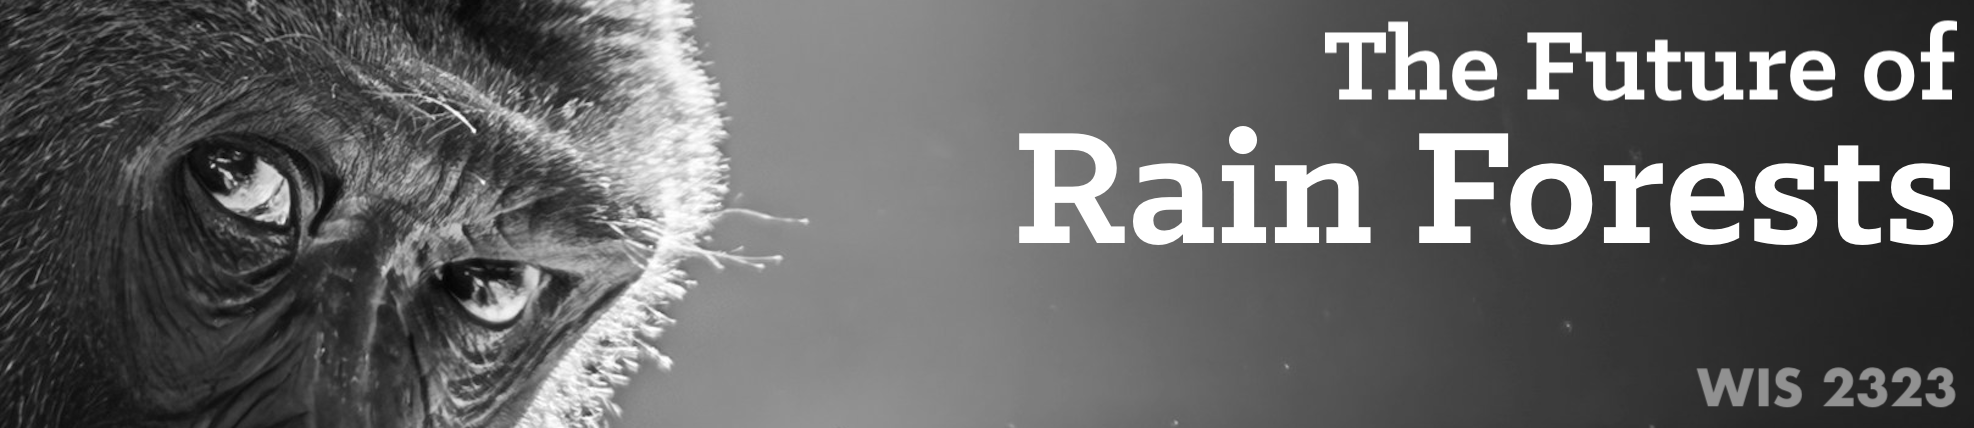
\includegraphics[keepaspectratio]{images/banner.png}}

This course investigates the fundamental issues addressed by scientists
studying tropical rain forests, including what gave rise to their
remarkable biodiversity, the drivers and consequences of deforestation,
why people are fascinated by rain forests, cultural stereotypes about
the tropics, and if forest conservation is compatible with socioeconomic
development. \textbf{\emph{By the end of the course students will be
able to:}}

\begin{itemize}
\tightlist
\item
  Recognize and describe stereotypes about rain forests \& their
  residents
\item
  Analyze rain forest tropes in art, literature, \& popular culture
\item
  Discuss \& evaluate hypotheses for the origins and maintenance of
  tropical biodiversity
\item
  Explain \& compare human history in rain forests
\item
  Review contemporary threats to rain forests
\item
  Analyze and visualize data on deforestation
\item
  Review and contrast strategies for rain forest conservation \&
  restoration
\item
  Identify rain forests in their daily lives \& set personal goals for
  advancing their conservation
\item
  Produce materials for communicating about rain forests to family and
  peers
\end{itemize}

\subsection*{When \& Where}\label{when-where}
\addcontentsline{toc}{subsection}{When \& Where}

\textbf{When:} Tuesdays 3:00-3:50 and Thursdays 3:00-4:55\\
\textbf{Where:} LIT 0231 (both days)

\subsection*{Instructor \& TA}\label{instructor-ta}
\addcontentsline{toc}{subsection}{Instructor \& TA}

\textbf{Instructor:} Dr.~Emilio M. Bruna {[}embruna@ufl.edu, (352)
846-0634{]}\\
\textbf{Teaching Assistant:} Priyanka Hari Haran {[}phariharan1@ufl.edu,
(352) 846-0527{]}

\subsection*{Credits \& Prerequisites}\label{credits-prerequisites}
\addcontentsline{toc}{subsection}{Credits \& Prerequisites}

\textbf{Credits:} 3\\
\textbf{Prerequisites:} None\\
\textbf{Quest Program:} Quest 2 \\
\textbf{GenEd Designation:} International

A minimum grade of C is required for Quest and General Education credit.
Courses intended to satisfy Quest and General Education requirements
cannot be taken S-U.

\subsection*{Minors \& Certificates}\label{minors-certificates}
\addcontentsline{toc}{subsection}{Minors \& Certificates}

This course counts towards:

\begin{itemize}
\tightlist
\item
  The Minor \& Certificate in Latin American Studies. See
  \url{https://www.latam.ufl.edu/academics/undergraduate-programs} for
  more information.
\end{itemize}

\bookmarksetup{startatroot}

\chapter{Required Materials}\label{required-materials}

\textbf{Materials and Supplies Fees}: None.

\textbf{Textbooks to purchase:} None.

\begin{itemize}
\item
  All materials, including readings and videos, will be made available
  on the course Canvas page. \bigskip
\item
  \emph{Students should sign up for free online access to the New York
  Times and Wall Street Journal by following the instructions at
  \href{https://businesslibrary.uflib.ufl.edu/c.php?g=943928&p=7708734}{this
  UF Libraries Website}} \footnote{Some of the assigned readings from
    these sources have dynamic multimedia data visualizations or video
    that can't be appreciated in the \texttt{.pdf} versions posted to
    canvas.}.
\end{itemize}

\begin{center}\rule{0.5\linewidth}{0.5pt}\end{center}

\bookmarksetup{startatroot}

\chapter{Office Hours}\label{office-hours}

\subsection*{When}\label{when}
\addcontentsline{toc}{subsection}{When}

\begin{itemize}
\item
  \textbf{Instructor:} Wednesday \& Friday 1:30-3:00 pm or by
  appointment. I am happy to meet either in-person or online. You can
  drop- or log-in at any time during the session or guarantee a specific
  time slot by signing up for a specific time here:
  \url{https://embruna.youcanbook.me}.
\item
  \textbf{Teaching Assistant:} Tuesday 1:00-2:30 pm or by appointment
  (in-person \& online).
\end{itemize}

\subsection*{Where}\label{where}
\addcontentsline{toc}{subsection}{Where}

\begin{itemize}
\item
  \textbf{In-person:} The Tropical Ecology \& Conservation Lab is
  located next to the Rawlings Hall bus stop (711 Newell Drive, a 5
  minutes from Turlington Plaza). For a map to our location click the
  ``Contact'' link at \href{http://brunalab.org}{BrunaLab.org}).
\item
  \textbf{Online:} use the zoom link on the course Canvas page. We are
  online the entire session.
\end{itemize}

\begin{tcolorbox}[enhanced jigsaw, title=\textcolor{quarto-callout-tip-color}{\faLightbulb}\hspace{0.5em}{Can you give me \textbf{one good reason} why I should go to Office
Hours?}, left=2mm, coltitle=black, colback=white, opacitybacktitle=0.6, arc=.35mm, leftrule=.75mm, toprule=.15mm, toptitle=1mm, bottomtitle=1mm, colbacktitle=quarto-callout-tip-color!10!white, breakable, titlerule=0mm, bottomrule=.15mm, opacityback=0, rightrule=.15mm, colframe=quarto-callout-tip-color-frame]

I can give you \textbf{ten}.

\begin{enumerate}
\def\labelenumi{\arabic{enumi}.}
\tightlist
\item
  To introduce yourself.
\item
  Get clarification on assignments.
\item
  Argue about a topic that came up in class.
\item
  Grab a (free) tea, coffee, or espresso in our lab kitchen.
\item
  Make sure you understood the key points from a class session.
\item
  Ask for feedback on ideas for course projects.
\item
  Get advice on successfully navigating academic life at UF.
\item
  Discuss how to gain experience for your post-graduation goals.
\item
  Request help arranging a study group.
\item
  You don't need a good reason\ldots just come on by.
\end{enumerate}

\end{tcolorbox}

\begin{center}\rule{0.5\linewidth}{0.5pt}\end{center}

\bookmarksetup{startatroot}

\chapter{Grades \& Attendance}\label{grades-attendance}

Learning in our class is achieved with an diverse array of methods
ranging from data analysis to essays to projects. In most class sessions
you will also be working with small groups of students to complete an
in-class assignment that reinforces the major themes of the day's topic.
In keeping with the philosophy of the Quest program, this course also
has \emph{Experiential Learning and Self-Reflection Components}.

\begin{tcolorbox}[enhanced jigsaw, title=\textcolor{quarto-callout-tip-color}{\faLightbulb}\hspace{0.5em}{Important note regarding class discussions \& group work.}, left=2mm, coltitle=black, colback=white, opacitybacktitle=0.6, arc=.35mm, leftrule=.75mm, toprule=.15mm, toptitle=1mm, bottomtitle=1mm, colbacktitle=quarto-callout-tip-color!10!white, breakable, titlerule=0mm, bottomrule=.15mm, opacityback=0, rightrule=.15mm, colframe=quarto-callout-tip-color-frame]

We will explore some challenging, important problems and increase our
understandings of different perspectives and approaches for addressing
them. These conversations may not always be easy; we sometimes will make
mistakes in both how we communicate our perspective and what we hear
other say. There may be times when we need patience, courage,
imagination, and of course mutual respect to engage our texts,
classmates, instructors, guests, and our own ideas and experiences.
\emph{Disrespectful or disruptive behavior will not be tolerated}. And
always remember that as scholars we rely on critical thinking, data,
prior scholarship, and expert opinion when interrogating assigned
readings and discussing course content with classmates and instructors.

\end{tcolorbox}

\subsection*{Assignments (1000 pts)}\label{assignments-1000-pts}
\addcontentsline{toc}{subsection}{Assignments (1000 pts)}

\begin{center}
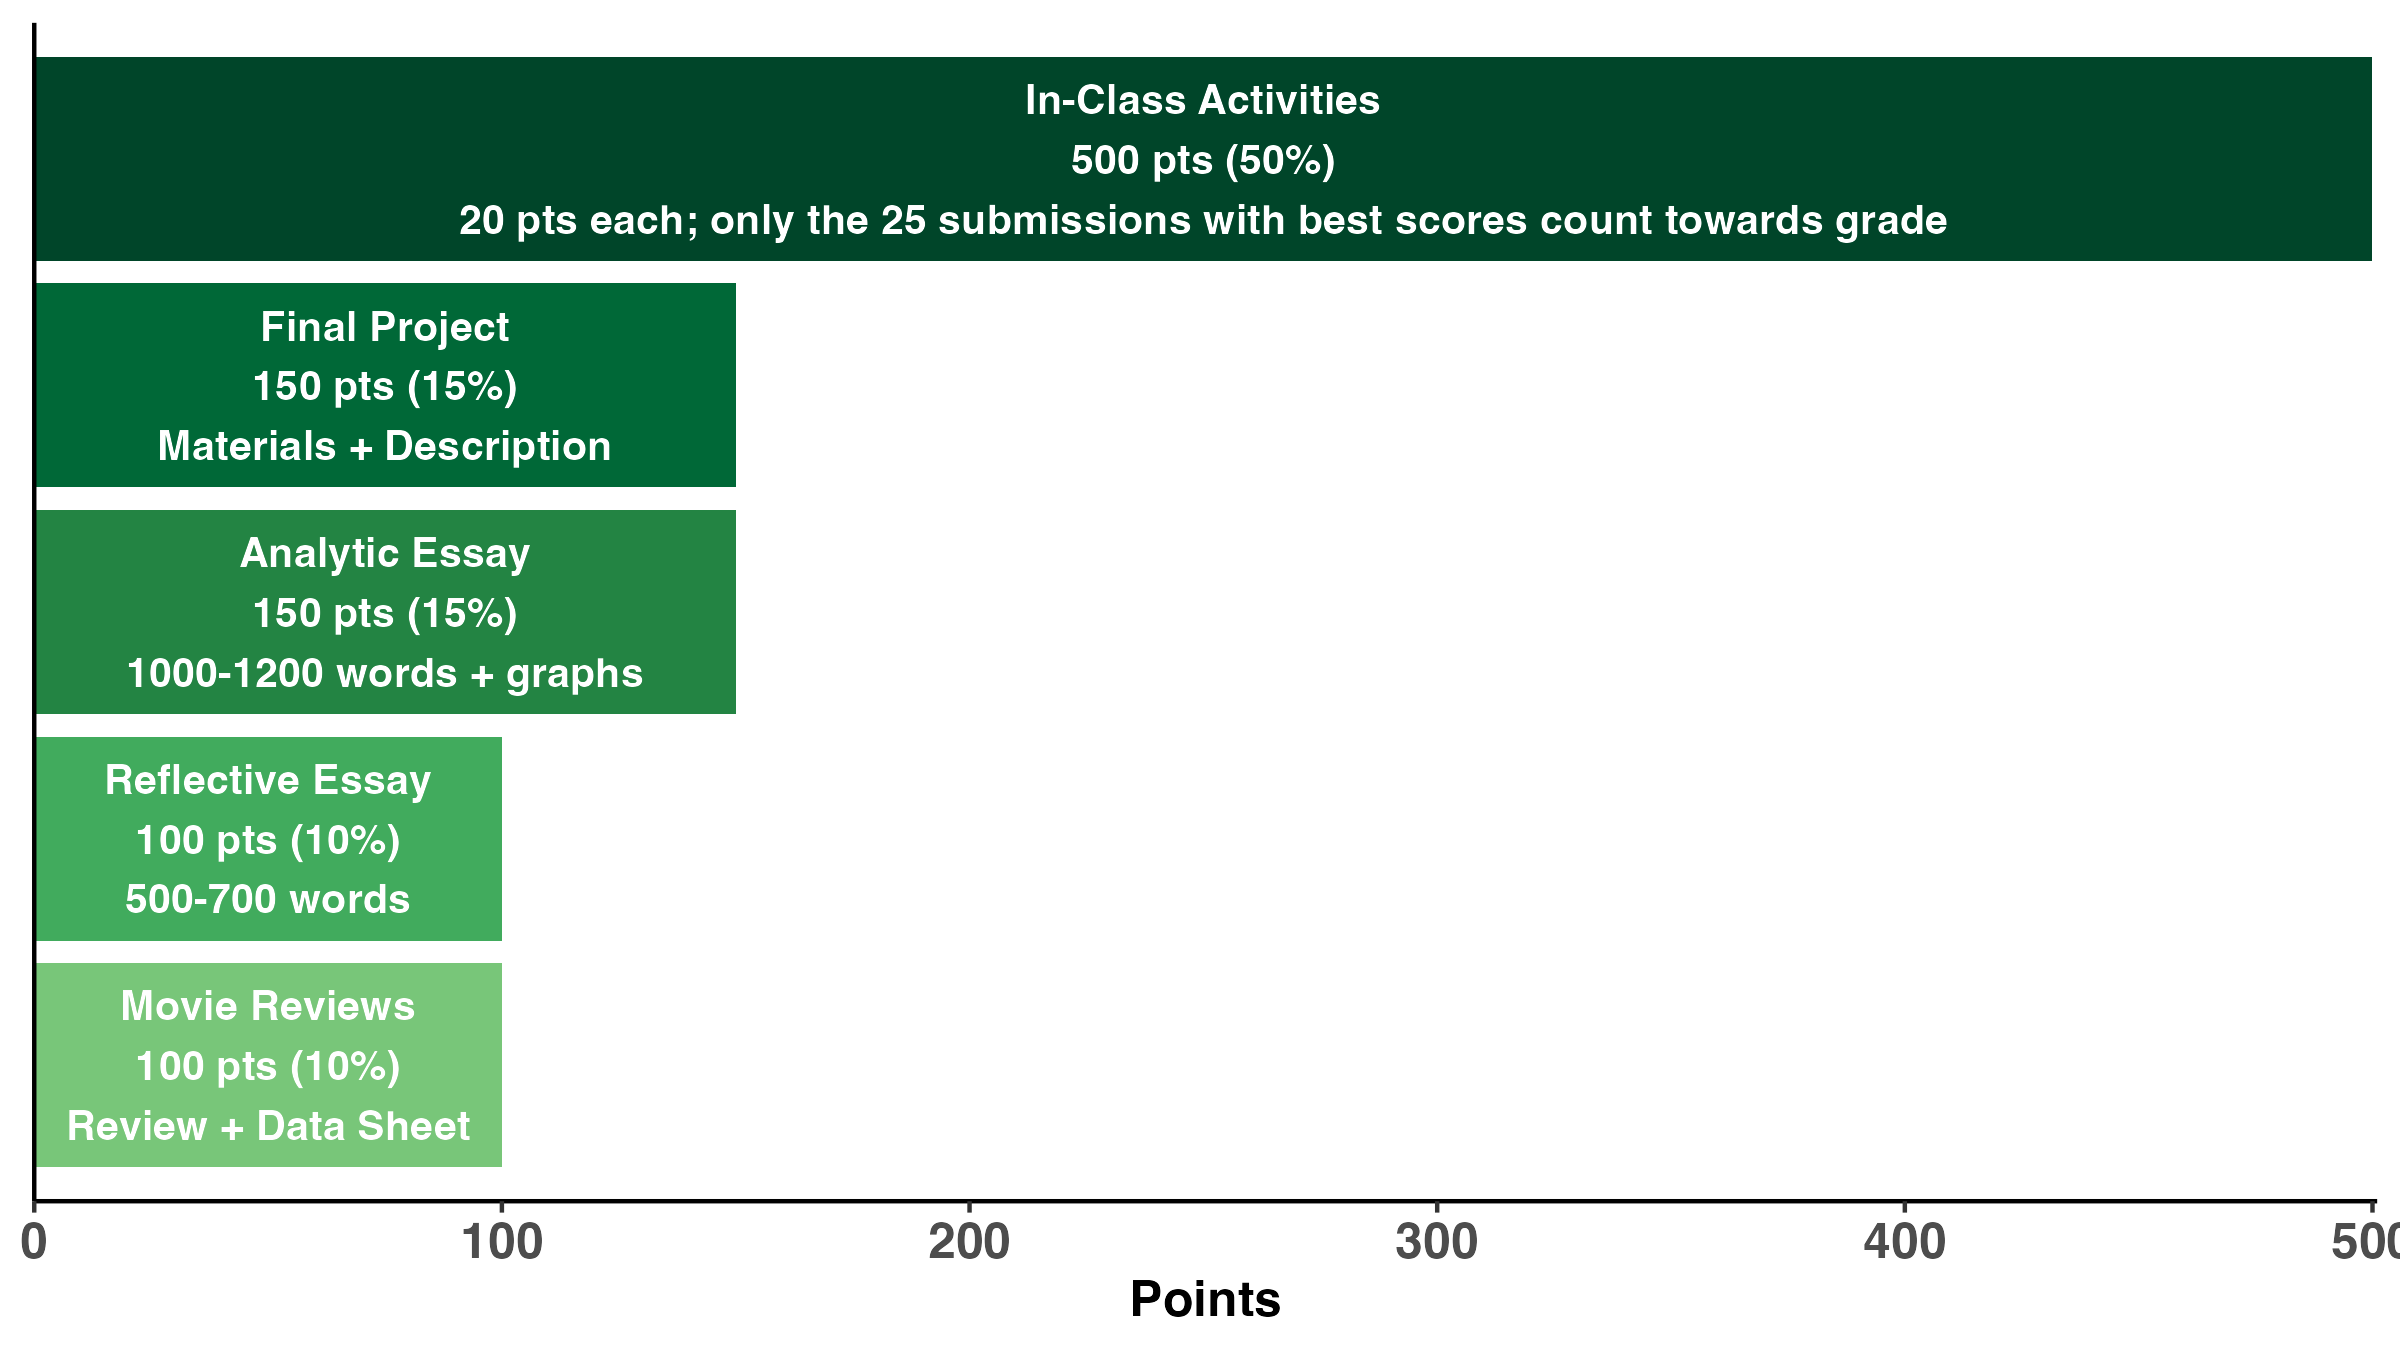
\includegraphics[width=1\linewidth,height=\textheight,keepaspectratio]{images/hw.png}
\end{center}

\subsection*{Grading}\label{grading}
\addcontentsline{toc}{subsection}{Grading}

\textbf{In-class Assignments are due by the following class session.}
Late assignments will lose 10 pts.

\textbf{\emph{Regrades:}} Requests for re-evaluation of assignments must
be accompanied by an explanation for why you think you deserve
additional credit and the number of additional points you think you
deserve. The deadline for submission is one week after the work was
returned.

\textbf{\emph{Grade Assignment}} (based on \% of total points earned): A
= 94--100\%, A- = 90--93\%, B+ = 87--89\%, B = 84--86\%, B- = 80--83\%,
C+ = 77--79\%, C = 74--76\%, C- = 70--73\%, D+ = 67--69\%, D = 64--66\%,
D- = 60--63\%, E\textless60

\textbf{\emph{Grade Points:}} For information on how UF assigns grade
points, visit:
\url{https://catalog.ufl.edu/UGRD/academic-regulations/grades-grading-policies/}

\subsection*{Attendance}\label{attendance}
\addcontentsline{toc}{subsection}{Attendance}

Though attendance is not required, many of the sessions we will be
completing activities in class that count towards your grade. Most of
these can be completed independently, but by doing them in class you
will benefit from working collaboratively with the other students.

\textbf{Some of the in-class activities can only be completed in that
day's class session.} If you miss class on one one of these days, that
is why the grade for in-class activities is based on a subset of the
total activities; you can also elect to make up lost points with
extra-credit assignments. \textbf{\emph{If you need to miss class for
any reason, please let me know as soon as possible}}. We will make
arrangements for you to complete any assignments and go over any
material you will be missing. I would much rather you focus on your
health, attend your conference, or support friends and family in need
than struggle to turn in assignments.

\subsection*{Participation}\label{participation}
\addcontentsline{toc}{subsection}{Participation}

Consistent informed, thoughtful, and considerate class participation is
encouraged (and in some cases required). \emph{If you have personal
issues that prohibit you from joining freely in class discussion (e.g.,
shyness, language barriers, medical condition): no problem.} let us know
and we will discuss alternative modes of participation.

\begin{center}\rule{0.5\linewidth}{0.5pt}\end{center}


\backmatter


\end{document}
